En este capítulo se describen los procesos de operación relacionados a los módulos hechos durante este trabajo terminal. \\

Se definieron los roles que se encargan de registrar la informacón por módulo así como el proceso general operativo. Los roles definidos son los siguientes:

\begin{itemize}
	\item {Encargado de registro de infraestructura}
	\item {Encargado de registro de unidades de aprendizaje}
	\item {Encargado de registro de profesores}
	\item {Encargado de registro de convocatorias de movilidad}
	\item {Encargado de registro de convocatorias de cursos}
\end{itemize}

\subsection{Proceso Operativo}

En la figura \ref{fig:macro} se muestra el macroproceso en donde intervienen los cinco encargados de los diferentes módulos, así como la interacción del alumno en los mismos. \\
De acuerdo al flujo mostrado en la figura \ref{fig:macro} se pueden tomar los siguientes cursos de acción:  

\begin{itemize}
	\item {Se puede realizar la gestión de los espacios y la gestión de convocatorias de movilidad sin necesidad de contar con información previa y terminar con el proceso.}
	\item {Posterior a la carga de información en el módulo de salones se puede pasar a la gestión de unidades de aprendizaje y a la gestión de cursos.}
	\item {Ya que se cuenta con información de espacios y de unidades de aprendizaje se puede gestionar profesores, dado que en el módulo se requiere información registrada en los módulos antes mencionados.}
\end{itemize}

\begin{figure}[h!]
	\begin{center}
		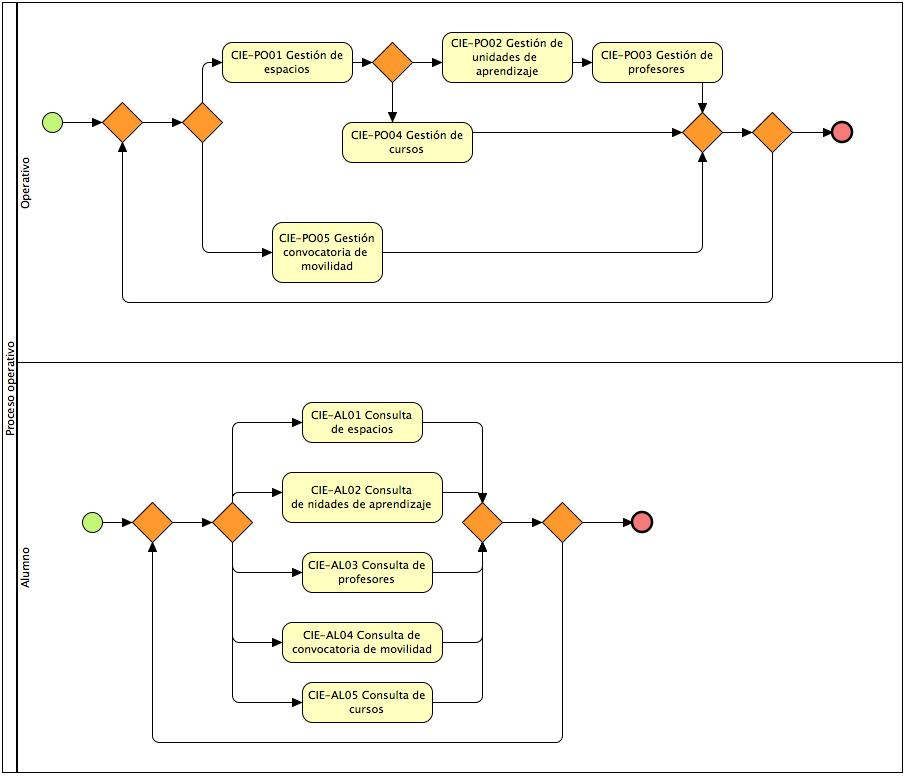
\includegraphics[width=1\textwidth]{images/procesos/macro.jpg}
		\caption{Proceso operativo.}
		\label{fig:macro}
	\end{center}
\end{figure}

En la parte baja del diagrama podemos ver el proceso del alumno para la consulta de información en los diversos módulos de la aplicación. El alumno puede seguir el flujo del diagrama en cualquier dirección y no cuenta con restricciones de consulta entre un módulo y otro.

\subsection{Proceso del encargado de registro de infraestructura.}

En la figura \ref{fig:espacios} se muestra el diagrama del proceso para el encargado de registro de infraestructura. 

\begin{figure}[h!]
	\begin{center}
		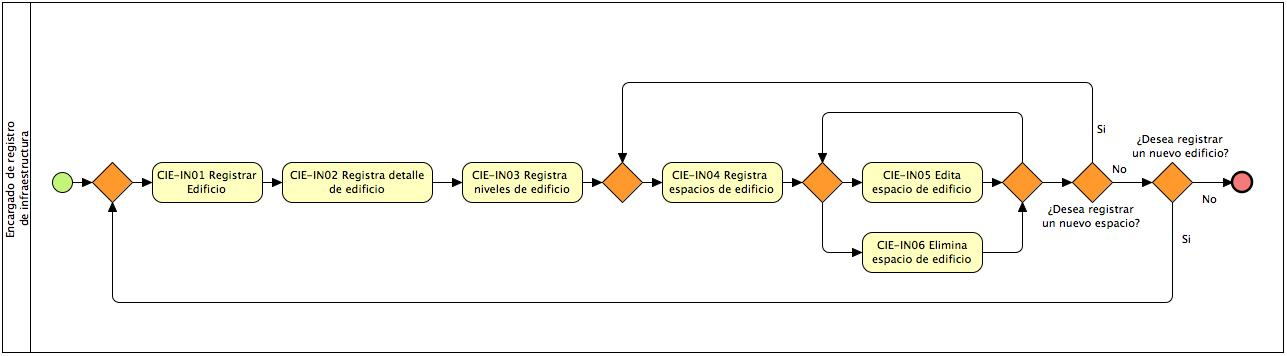
\includegraphics[width=1\textwidth]{images/procesos/espacios.jpg}
		\caption{Proceso del encargado de registro de infraestructura.}
		\label{fig:espacios}
	\end{center}
\end{figure}

\subsection{Proceso del encargado de registro de unidades de aprendizaje.}

\begin{figure}[h!]
	\begin{center}
		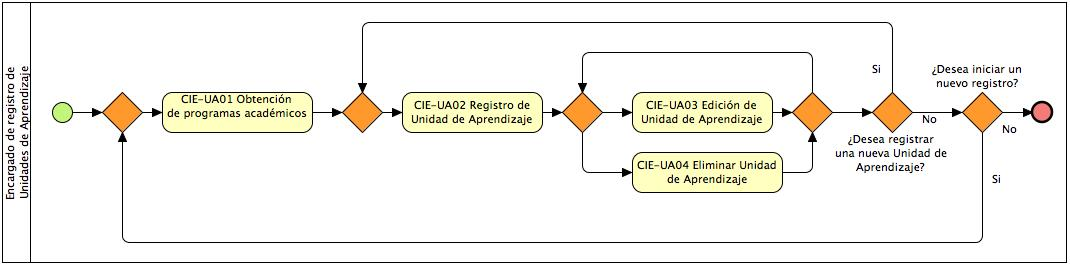
\includegraphics[width=1\textwidth]{images/procesos/unidades.jpg}
		\caption{Proceso del encargado de registro de unidades de aprendizaje.}
		\label{fig:unidades}
	\end{center}
\end{figure}

\subsection{Proceso del encargado de registro de profesores.}

\begin{figure}[h!]
	\begin{center}
		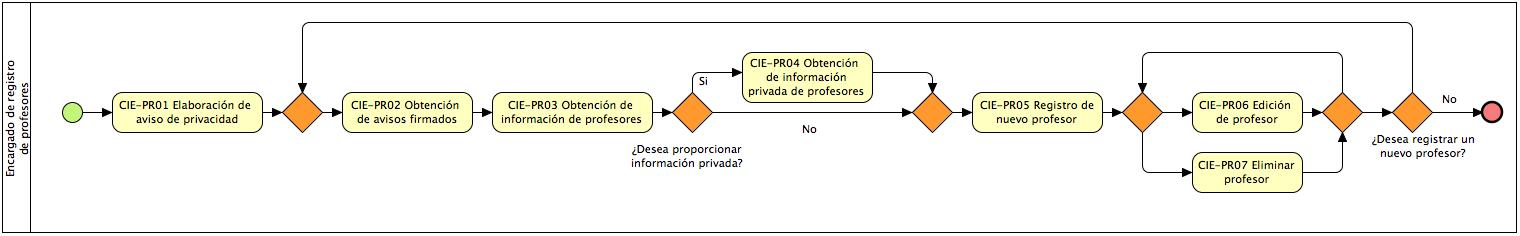
\includegraphics[width=1\textwidth]{images/procesos/profesores.jpg}
		\caption{Proceso del encargado de registro de profesores.}
		\label{fig:profesores}
	\end{center}
\end{figure}

\subsection{Proceso del encargado de registro de convocatorias de movilidad.}

\begin{figure}[h!]
	\begin{center}
		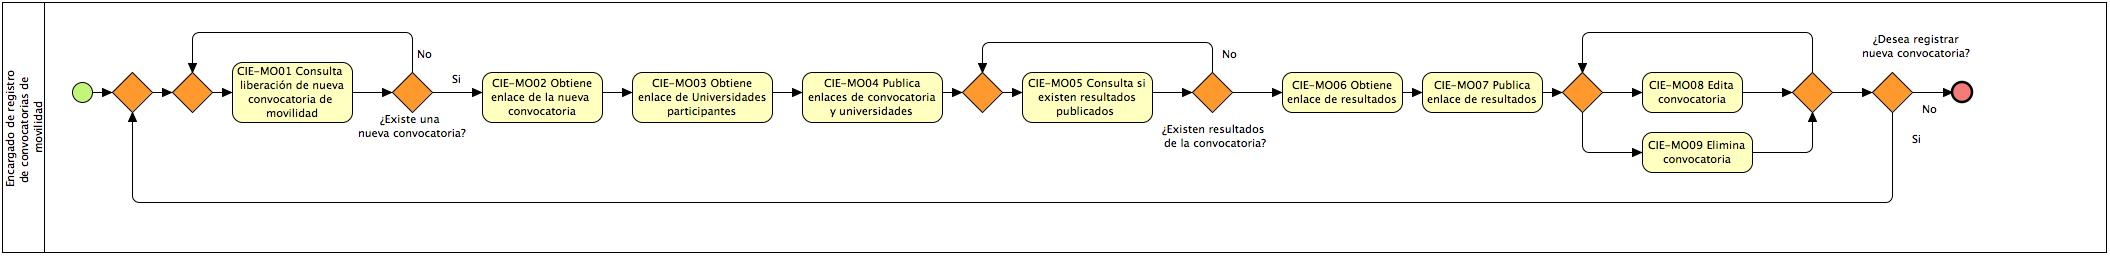
\includegraphics[width=1\textwidth]{images/procesos/movilidad.jpg}
		\caption{Proceso del encargado de registro de convocatorias de movilidad.}
		\label{fig:movilidad}
	\end{center}
\end{figure}

\subsection{Proceso del encargado de registro de convocatorias de cursos.}

\begin{figure}[h!]
	\begin{center}
		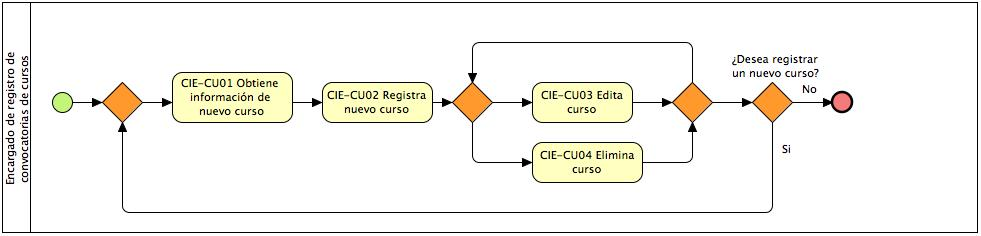
\includegraphics[width=1\textwidth]{images/procesos/cursos.jpg}
		\caption{Proceso del encargado de registro de convocatorias de cursos.}
		\label{fig:cursos}
	\end{center}
\end{figure}